\chapter{History of solid breeder design}\label{sec:solid-breeder-history}


\section{The Basics of Nuclear Fusion and Tritium Breeding}\label{sec:fusion-basics}

The fusion reaction chosen for the first demonstrable fusion power plants involves the two hydrogen isotopes of deuterium and tritium. The deuterium-tritium (DT) reaction has a high reaction probability at the lowest ion temperature and a high energy yield. Alternative fusion reactions of two deuterium atoms or a deuterium atom with helium-3 are advantageous in other regards, such as no radioactive byproducts or fuel availability, but their relatively-higher ion temperature preclude them from current feasibility.\cite{abdou} The DT reaction proceeds as
\begin{align}
	\mathrm{D} + \mathrm{T}&\xrightarrow{}\ ^4\mathrm{He}+\mathrm{n}+17.58\ \text{MeV} \label{eq:dt-reaction}
\end{align}

Of the two isotopes fused, deuterium ($D$, or $^2$H) is a stable isotope and is naturally occurring in an average abundance of 0.015 mole percent in water on Earth. To demonstrate just how plentiful deuterium is as a fuel source, there is approximately 100 million billion kilograms of deuterium in the Earth's oceans. If all energy on Earth were produced from DT fusion power plants, there would be enough deuterium to outlast the lifetime of our sun. It is safe to say we will not exhaust our deuterium sources on Earth.

Tritium ($T$, or $^3$H), however, is radioactive with a half-life of only about 12 years; any naturally occurring tritium decays at such a rapid pace it will never accumulate to an appreciable amount on Earth. If tritium is to be used as a fuel in a fusion power plant, it must be generated artificially. In-situ generation of tritium in a fusion reactor is possible with the assistance of lithium. Natural lithium will interact with neutrons as
\begin{subequations}\label{eq:lithium-t}
\begin{align}
	\mathrm{n} + \ ^7\mathrm{Li} &\xrightarrow \ \mathrm{n}+\alpha + \mathrm{T} -2.47\ \text{MeV}\label{eq:li7-t}\\
	\mathrm{n} + \ ^6\mathrm{Li} &\xrightarrow \  \alpha + \mathrm{T} +4.78\ \text{MeV} \label{eq:li6-t}
\end{align}
\end{subequations}
using the common short-hand of $\alpha$ in place of the helium nucleus. The cross-sections of the lithium reactions are given in Fig.~\ref{fig:li-xsects}. Of note in Fig.~\ref{fig:li-xsects} is the exothermic lithium-6 reaction (a neutron of any energy will incite the transmutation) and the threshold energy required of the incident neutron to incite the endothermic lithium-7 reaction. The exothermic reaction, in addition to producing tritium, is also the source of energy that will ultimately generate the electricity of the fusion power plant.

\begin{figure}[ht]
	\centering
	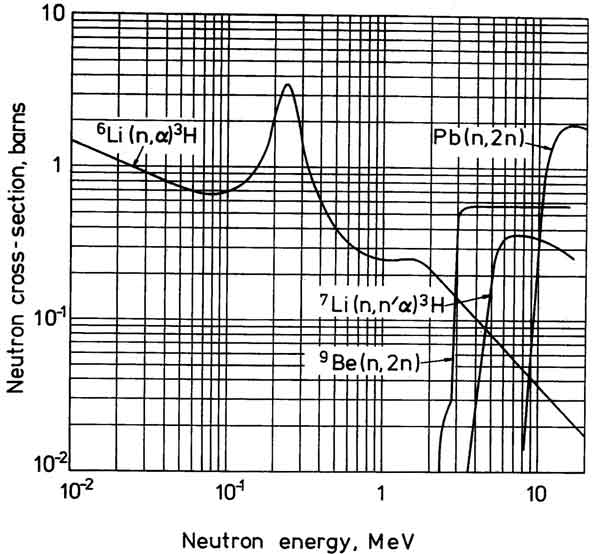
\includegraphics[width=\singleimagewidth]{chapters/figures/breeding_xsecs} 
	\caption{Cross-sections of various blanket materials. Note the threshold for the $^7$Li and neutron multiplying reactions.}
	\label{fig:li-xsects}
\end{figure}

Fortunately, lithium, like deuterium, is quite abundant on Earth. There is enough lithium accessible in the Earth's crust to generate tritium for 30 million years worth of DT reactions.\cite{Chen2011}. Thus lithium is an excellent candidate for generating the tritium necessary to self-sustain the fusion reaction in a power plant. Fusion reactor designs include so-called tritium breeding blankets which surround the plasma volume with lithium, however the form of lithium as it exists in the breeding blanket is a source of continued research.


A design was proposed by Abdou\etal\cite{Abdou1975} in 1975 wherein the plasma would be surrounded by a blanket of nonmobile, solid lithium. To exist in solid form at high temperatures, pure lithium, which has a melting temperature of only about 180~\celsius, must be combined with refractory materials (melting temperatures >1000~\celsius). To date, most parties researching solid breeder blankets have settled on lithium orthosilicate (\lis) or lithium metatitanite (\lit) as candidate ceramics.


At present there are two main concepts for tritium breeder designs: those containing liquid or solid lithium. Many of the functional requirements are similar between the two designs but their implementations are quite different. While much research has been -- and continues to be -- performed on the liquid breeder design (for examples, see Refs.~\cite{Hartmann1937,Hunt2006,Shercliff1953,Sommeria1982,Xv1937,Alfve1942}), the work of this dissertation focuses solely on the reference solid breeder design. In the next section, while introducing the breeding blanket, I will refer to the blanket almost exclusively as simply ``solid breeder'' though it should be understood that many of the generic features and requirements of the solid breeder are shared with its sister design, the liquid breeder.

As nuclear energy is deposited into the solid breeder, large thermal gradients in the solid lithiated ceramics will induce thermal stresses across large characteristic lengths. Avoiding thermal stress has led to most solid breeder designs implementing packed beds of small, spherical (or near-spherical) pebbles.\cite{Lulewicz2002, Mandal2012a, Tsuchiya1998, Cho2012} Moreover, tritium diffusion and release considerations for solid lithium ceramic support the choice of short characteristic lengths of individual pebbles. From an engineering design standpoint, the choice of packed bed has other desirable characteristics. For instance, the ensemble of small spherical pebbles can be filled into many complex shapes with relatively uniform porosity. The uniform packing of spheres permits a well-distributed flow of purge gas for tritium extraction. 

The advantages of the pebble bed design include ease of uniformly assembling the solid into complex geometries, ease of tritium extraction from the porous bed via an interstitial purge of helium, and with the small size of pebbles being more resilient to thermal stresses than a solid brick of lithiated ceramic.\cite{Casadio2004} 


Lithium oxide had been considered because of its favorable lithium density, among other attractive features, though the reaction of lithium with elemental oxygen is a concern. Pure lithium reacts with oxygen exothermically in reactions such as

\begin{subequations}
\begin{align}
	2\mathrm{Li} + \frac{1}{2}\mathrm{O} &\rightarrow \mathrm{Li}_2\mathrm{O} - 142.75\ \text{kCal/mol}\\
	2\mathrm{Li} + \mathrm{O} &\rightarrow \mathrm{Li}_2\mathrm{O}_2 - 151.9\ \text{kCal/mol}
\end{align}
\end{subequations}

Of primary concern in lithium fires is the peak flame temperature. This will determine, to a large extent, whether many radioactive species become air-borne by vaporization. The flame temperature depends on many variables. Some investigations found it to be about 2500~K which would cause some materials to melt but not vaporize. [cite Abdou's class notes?]